\part{Proposta}
  \chapter{Como criar produtos com qualidade?}
    Quando produzimos um \textit{software}, focamos sempre nas funcionalidades que
    o sistema deve conter, pretendemos entregar o mais rápido possível e respeitar
    as datas alinhadas com o negócio. Porem, na pressa de colocar as funcionalidades
    em produção, desconsideramos os requisitos não-funcionais e por mais que a
    funcionalidade tenha sido entregue conforme o específicado, o usuário não
    consegue utiliza-la, consequentemente, está entrega não está gerando valor. \newline
    Mas como assim, os requisitos foram atendidos mas o usuário não consegue utilizar?
    Como ignoramos os requisitos não-funcionais, o usuário pode estar sofrendo por
    diversos problemas, por exemplo, um \textit{layout} confuso, um desempenho baixo,
    o sistema está forçando ele a realizar uma tarefa que ele não está acostumado a
    fazer, ou pelo menos não no momento em que apareceu no sistema. Como entregamos
    vizando a data da entrega e nãp o valor para o usuário, aceitamos o risco de
    entregar algo que o usuário não vê valor, e por diversas vezes cometemos erros.
    Ao testar uma funcionalidade, não costumamos ter a visão total do negócio,
    focamos na funcionalidade, então questões como tempo de resposta, ordem lógica
    no processo, localização das informações, nos passam despercebidos, não estamos
    utilizando o sistema diariamente para entender estas questões sozinhos, e o
    negócio muda frequentemente, então quando finalmente entendemos a realidade do
    usuário, ela já mudou, e voltamos a estar sucetiveis ao erro. \newline
    Como não atendemos a expectativa do usuário, e a funcionalidade não está gerando
    valor, implementamos diversas melhorias, todas o mais rápido possível, o que
    acaba gerando \textit{bugs}, como erramos uma vez, precisamos corrigir o erro
    o mais rápido possível, o que nos faz ignorar novamente requisitos não-funcionais
    e, por sua vez, ignoramos questões de arquitetura de \textit{software} o que
    acaba deixando o sistema mais complexo, dificulta a sua manutenção, e deixa o
    sistema mais sucetível a erros. \newline
    Não queremos mais cometer estes erro, queremos cria o produto perfeito que
    será totalmente aderente ao usuário e que irá gerar valor para o negócio. \newline
    O primeiro passo para gerar um produto de qualidade, que auxilia a empresa a
    concluir os seus objetivos e que traga valor ao negócio e entender que não
    existe produto perfeito. Somos humanos, erramos constantemente, realizamos
    escolhas erradas, nos equivocamos. Para realizar uma entrega de pouco risco
    e extremamente acertiva, é necessário muito tempo de planejamento e de estudo,
    como por exemplo a construção de uma avião, ou de um prédio, ou de um
    equipamento hospitalar, este tipo de produto não pode ter falhas, pois caso
    tenha, é um risco para a vida das pessoas. Porem, nosso negócio é mais
    dinâmico, as necessidades muda com mais frequência do que as necessidades de
    um avião, se utilizarmos tanto tempo para planejar como podemos seguir as
    mudanças do negócio?

    \section{Assumindo riscos}
      Para conseguirmos acompanhar o negócio e gerar valor para a empresa, evemos
      escolher os riscos que vamos enfrentar. Mesmo um avião encara riscos em seu
      projeto, por isso que é implementado diversas redundancias nas funcionalidades
      mais importantes. Devemos pensar de forma semelhante, qual o objetivo do nosso
      projeto? Qual é sua funcionalidade mais importante? Quais são os riscos que
      vamos encarar? \newline
      Com base nisso, podemos focar a maior parte de nosso tempo no \textit{core}
      do produto, descobrindo o objetivo do sistema, podemos alinhar com os objetivos
      da empresa, assim gerando o retorno esperado. Para realizar o levantamento
      da funcionalidade é importante considerar o nome da funcionalidade, a sua
      importância, os objetivos em que ela vai nos auxiliar a alcançar, os riscos
      que vamos enfrentar com ela e as dependências para disponibilizar a
      funcionalidade ao usuário.

      \begin{table}[h!]
        \centering
        \begin{tabular}{|c|p{10cm}|}
          \hline
          \textbf{Funcionalidade} &
          Nome da funcionalidade que será desenvolvida. \\ \hline
          \textbf{Importância} &
          A importância que a funcionalidade representa para o negócio, separa entre
          alta, média e baixa. \\ \hline
          \textbf{Objetivos} &
          Os objetivos que está funcionalidade irá auxiliar à alcançar. \\ \hline
          \textbf{Riscos} &
          Quais os riscos que essa funcionalidade pode gerar para o negócio. \\ \hline
          \textbf{Dependências} &
          Quais são as dependências para a utilização e desenvolvimento dessa
          funcionalidade. \\ \hline
        \end{tabular}
        \caption{Definição da classificação de funcionalidaes}
        \label{Tabela:1}
      \end{table}

      Toda funcionalidade deve ter um nome que represente o que será desenvolvido
      pois, durante o desenvolvimento, é através do nome que os desenvolvedores
      vão se comunicar, sem um nome claro, que represente bem o negócio, os
      desenvolvedores não vão conseguir se comunicar de forma clara para entender
      as necessidades do negócio. Termos e nomeclaturas devem ser estabelecidas,
      para que o usuário entenda como o sistema deve ser utilizado e para os
      desenvolvedores compreenderem como o sistema será utilizado. Através desta
      comunicação, o time de desenvolvimento consegue extrair os requisitos de forma
      mais fácil e formular um padrão de qualidade. \newline
      É necessário colocar a importância da funcionalidade que será desenvolvida pois,
      com base nela podemos entender a ordem que vamos iniciar o desenvolvimento
      e quais os riscos podemos enfrentar e através da importância podemos definir
      o rigor dos testes que devemos realizar no desenvolvimento da funcionalidade
      e o padrão de qualidade para cada nível de importância. Embora colocamos
      somente três níveis de importância (alto, médio e baixo), cada negócio pode
      ter mais níveis, porém recomendamos não exagerar e passar de cinco níveis,
      pois o principal objetivo desta classificação é forçar escolhermos quais
      funcionalidades são realmente mais importantes, se colocarmos muitos níveis,
      a menor classificação será "alta". \newline
      As funcionalidades que vamos desenvolver tem que estar relacinada com um
      objetivo da empresa, pois é isso que dá propósito para ela, e a nossa base
      para verificar se ela está gerando valor. Com base no uso da funcionalidade,
      podemos verificar se o objetivo está sendo alcançado, e com base nesse
      retorno, podemos decidir quais serão os nossos próximos passos. \newline
      Quando pensamos em uma funcionalidade, devemos sempre considerar os riscos
      para o negócio, a utilização de um sistema implica em com a operação da
      empresa trabalha, e toda mudança gera riscos para a operação. Tudo que é
      novo, deve ser ensinado, por mais que a funcionalidade reflita exatamente o
      que os usuários já faziam, eles vão começar a eecutar essas atividades em
      um outro lugar, o que no começo pode gerar dúvidas e frustrações. Devemos
      sempre levantar os riscos com base na perspectiva do usuário, pois assim
      podemos entender quais serão as reações delese e quais estratégias devemos
      utilizar para engajar o uso da ferramenta e buscar por melhorias. \newline
      Com base nos objetivos, nas funcionalidades e nos riscos, podemos mapear as
      pendências das funcionalidades, onde conseguimos traçar quais os passos que
      devemos tomar para iniciar o desenvolvimento até disponibilizar a funcionalidade
      para o usuário. \newline
      Para o levantamento dessas informações recomendamos utilizar o formato de
      tabela. A tabela possibilita consolidar de forma clara cada tópico e sempre
      que a empresa tiver um novo objetivo, é mais fácil analisar o que já foi listado,
      possibilitando ver se o sistema se encaixa com essa nova necessidade ou se será
      necessário uma nova funcionalidade, ou se será necessário um novo produto,
      ou uma reformulação do negócio. Quando listamos tudo que estamos fazendo
      junto com o que o negócio pretende alcançar, podemos tomar decisões mais
      acertivas, entender dependências e otimizar o valor que será desenvolvido.
      Muitas vezes focamos em desenvolver uma funcionalidade que não irá gerar
      muito valor para o negócio, o que nos faz aceitar um risco que não precisamos
      no momento, toda funcionalidade gera riscos, então é melhor nos concentrarmos
      somente naqueles que podem gerar mais valor. \newline
      Uma vez definido nossas funcionalidade, sua importância e os objetivos que
      pretendemos com elas, podemos escolher quais vamos implementar primeiro e
      quais riscos nós vamos enfrentar. \newline
      Para exemplificar a utilização da tabela proposta vamos considerar uma
      empresa que possuí vendores que entram em contato com outras empresas para
      negociar a venda de computadores. Estes computadores podem ser customizados
      pelo cliente, solicitando maior espaço de memória, se deseja um computador
      com \textit{SSD} ou \textit{HD}, qual o processador, entre outras ecolhas.
      Embora já existam computadores pré-montados, eles podem ser customizados
      somente aproveitando a base do produto. \newline
      Hoje a venda é feita sem a utilização de um sistema, a especificação que o
      cliente deseja é feita de forma indivídual por cada vendedor e controlado por
      meio de planilhas, onde cada vendedor possui a sua forma de organizar. Somente
      o pedido final é colocado em um sistema de controle de pedidos, para emitir a
      nota. A comunicação entre os vendedores e a área técnica é feita por meio de
      telefone e email, os produtos base e os produtos vendidos são compartilhados
      através de planilhas enviadas por email. Como cada vendedor negocia de uma
      forma, nã há Padronização nas planilhas, o que acaba gera confusões na área
      técnica na hora da montagem dos produtos. Outro ponto a destacar é que a área
      administrativa não tem visibilidade de como as negociações estão sendo realizadas
      o que dificulta o entendimento do negócio como um todo e a cração de
      estratégias. \newline
      Com base nessas necessidades, a empresa decidiu começar um projeto para a
      criação de um sistema para os vendedores realizar as suas negociações.
      Onde o produto base seria disponibilizado na ferramenta e os pedidos finais
      seriam montados conforme a negociação avança. Outra necessidade, é que a
      negociação deve ser faseada, para que seja possível rastrear os passos do
      vendedor e ter uma melhor visão do negócio. \newline
      Neste cenário, o primeiro passo é levantar as princípais funcionalidades para
      atender o negócio, já colocando a sua importância e os objetivos que pretendemos
      alcançar.

      \begin{table}[h!]
        \centering
        \begin{tabular}{|c|c|p{8cm}|}
          \hline
          \textbf{Funcionalidade} &
          \textbf{Importância}  &
          \textbf{Objetivos} \\ \hline
          %Funcionalidade
          Cadastro de produtos &
          %Importância
          Alta &
          %Objetivos
          Padronização na criação de produtos; \newline
          Reduzir o cadastro incorreto de produtos.
          \\ \hline
          %Funcionalidade
          Venda de produtos &
          %Importância
          Alta &
          %Objetivos
          Venda faseada do produto; \newline
          Melhor rastreabilidade da venda; \newline
          Padronização da negociação.
          \\ \hline
          %Funcionalidade
          \textit{Chat} interno &
          %Importância
          Baixa &
          %Objetivos
          Otimização da comunicação entre a área técnica e os vendedores.
          \\ \hline
        \end{tabular}
        \caption{Exemplo de levantamento de funcionalidades}
        \label{Tabela:2}
      \end{table}

      Na tabela dois, representamos três funcionalidades, o cadastro de produtos,
      a venda de produtos, e o \textit{chat} interno. Podemos notar que a maior necessidade
      da empresa é a de padronizar a venda do produto, onde a negociação deve ser
      feita de forma mais uniforme e que facilite os vendedores a venderem produtos
      mais aderentes com o que a área técnica consegue produzir. Com base nestas
      necessidades, foi levantado as funcionalidades de cadastro de produtos e
      venda de produtos, onde o cadastro está relacionada com a padrinização da
      criação do produto e a venda está relacionada com a padronização da venda.
      Porem, a funcionalidade de \textit{chat} interno, não é uma prioridade para
      o negócio, as áreas estão se comunicando, o problema é que cada vendedor
      trabalha de um jeito, o que dificulta as decisões da área técnica. Embora um
      dos objetivos seja melhorar a comunicação entre as áreas, este não é o maior
      dos problemas que precisamos resolver, então os riscos que desta funcionalidade
      não precisam ser corridos até o desenvolvimento das outras duas. \newline
      Outro ponto de destaque é a identificação das dependências, quando mapeamos
      as dependências, conseguimos ver qual funcionalidade precisamos realizar
      primeiro, como listado no exemplo, não é possível vender os produtos sem antes
      cadastrá-los. Mas alem da dependências entre funcionalidades, podemos listar
      o que precisamos fazer para disponibilizar a funcionalidade para o usuário,
      como apresentado no exemplo, todas as funcionalidades precisam de treinamento,
      como o sistema é novo e cada vendedor realiza as negociações do seu jeito,
      é importante explicar como foi montado o processo de vendas e apresentar
      como realizar as atividades no sistema. \newline
      Cada funcionalidade tem os seus riscos, porem é através de sua importância que
      podemos criar estratégias para enfrentar estes riscos e marcar estas ações
      que definimos em nossa estratégia como dependências para liberar o uso da
      funcionalidade, é importante atrelar estas ações como dependências, pois desta
      forma os usuários não são surprendidos, e é através dos treinamentos e das
      apresentações que podemos pegar o \textit{feedback} dos usuário e começar a
      mapear novas funcionalidades e melhorias. Podemos ver o mapeamento dos riscos
      e das dependências das funcionalidades exemplo na tabela três.\newline

      \begin{table}[h!]
        \centering
        \begin{tabular}{|c|p{4cm}|p{6cm}|}
          \hline
          \textbf{Funcionalidade} &
          \textbf{Riscos}  &
          \textbf{Dependências}
          \\ \hline
          %Funcionalidade
          Cadastro de produtos &
          %Riscos
          Processo de cadastro de produtos mais demorado; \newline
          Criação de produtos menos flexível. &
          %Dependências
          Treinamento para cadastrar os produtos no sistema;\newline
          Explicação das regras utilizadas para o cadastro dos produtos.
          \\ \hline
          %Funcionalidade
          Venda de produtos &
          %Riscos
          Venda menos flexível; \newline
          Mudança na forma de negociação dos vendedores; &
          %Dependências
          Funcionalidade de cadastro de produtos; \newline
          Treinamento para realizar vendas no sistema; \newline
          Explicação das fases na venda.
          \\ \hline
          %Funcionalidade
          \textit{Chat} para clientes &
          %Riscos
          Não adoção do \textit{chat} como princípal meio de comunicação; \newline
          Utilização do \textit{chat} para assuntos sem relação ao trabalho; &
          %Dependências
          Treinamento para a utilização do \textit{chat}; \newline
          Treinamento sobre como se comunicar por \textit{chat}.
          \\ \hline
        \end{tabular}
        \caption{Exemplo de levantamento dos riscos e dependências por funcionalidade}
        \label{Tabela:3}
      \end{table}

    \section{Entendendo os requisitos de uma funcionalidade}
      Após entendermos os ricos, escolher quais vamos aceitar e definir a prioridade
      das funcionalidades que queremos desenvolver, devemos começar a refinar cada
      uma e definir quais são seus requisitos. É importante salientar que os
      requisitos, assim como foi com os riscos, devem partir do negócio, para assim
      fazer parte do sistema, a funcionalidade deve solucionar um problema e facilitar
      a vida dos usuários, agregando valor para o cotidiano deles e consequentemente
      agregando valor para o negócio. \newline
      A funcionalidade deve ser desenvolvida com base no que os usuários já fazem
      no dia a dia, temos que mapear todas as tarefas que o usuário executa,
      identificando quais incomodam e quais não incomodam. Identificando quais tarefas
      o usuário não gosta de fazer, já é um ponto de partida no que o sistema
      automatizar, uma vez que o usuário não precise fazer determinada funcionalidade,
      já facilitou o seu cotidiano. Outro ponto de atenção, são com as tarefas que
      o usuário não se importa em executar, automatizar ou mudar a forma que ele
      executa pode ser um problema em um promeiro momento, pois ele terá que se
      acostumar com uma nova forma de trabalho. Muitas vezes esse tipo de mudança
      pode se originar em uma nova fase da empresa, que está revendo os seus processos
      e mudando a forma como de trabalho dos colaboradores, neste caso, é importante
      implementar a funcionalidade de forma que seja um meio termo entre o que os
      usuários realizavam e a nova forma da empresa, desta forma os usuários
      começam a se adaptar a nova perspectiva e conforme o projeto for avançando,
      podemos ir adaptando a funcionalidade a restruturação da empresa. Devemos
      lembrar que nenhuma mudança acontece do dia para a noite, e uma mudança
      brusca na forma de trabalho pode gerar desconforto nos usuários e deixar eles
      confusos em como executar suas atividades. \newline
      Uma funcionalidade deve sofrer melhorias constantes, como o negócio está
      constantemente sofrendo mudanças, o sistema deve se adaptar para os novos
      requisitos do mercado, por este motivo, os requisitos devem ser identificados
      mas não podem ser considerados como certeza, o sistema deve estar pronto para
      sofrer qualquer tipo de alterações e a qualquer hora porem, sabemos que certas
      mudanças levam muito tempo e até a alteração, o requisito já sofreu mais uma
      alteração, por este motivo, devemos classificar nossos requisitos em nível
      de importância e em nível de mutabilidade. Enquanto nos riscos nós classificamos
      a funcionalidade como um todo, aqui vamos classificar os requisitos que formam
      essa funcionalidade, devemos sempre pensar, o que é essencial para a funcionalidade
      atingir o objetivo? O que pode se tornar uma melhoria para o futuro? Desta
      forma, conseguimos entregar valor mais rápido para diferentes áreas do negócio,
      pois se focarmos todo o nosso tempo na funcionalidade mais importante, nunca
      vamos realizar as outras funcionalidades. Para cada funcionalidade devemos
      tambem atribuir um nível de mutabilidade, ou seja, qual é a chance dessa
      funcionalidade sofrer alterações conforme o tempo vai passando, embora o
      negócio esteja em constante mudança, sabemos que certos processos dificilmente
      sofrem alterações, pois faz parte do \textit{core} da empresa, é a essência
      do negócio. A forma de classificar a mutabilidade é através de porcentagem,
      onde as primeiras classificações serão intuições com base na perspectiva do
      negócio, mas as seguintes, é importante que conforme o sistema vá sofrendo
      alterações e melhorias, estas taxas sejam atualizadas por funcionalidade.
      A primeira regra na hora de classificar é que não existe zero porcento, toda
      funcionalidade pode sofrer alterações, mesmo que demore anos para isso acontecer,
      a sociedade muda, novas tecnologias vão surgindo e o que era comum é subtituido
      por algo novo, que acaba se tornando o novo comum, e se a empresa não estiver
      preparada para acompanhar essas mudanças, ela acaba se perdendo no tempo.
      Realizando essa classificação podemos identificar quais processos estão
      consolidados e quais processos ainda devem ser estruturados, com essa visão
      sobre os processos, podemos identificar o novo \textit{core} do negócio e
      desta forma trabalhar em uma tranformação na empresa para atender as novas
      necessidades do mercado, assim evoluindo o sistema ou até mesmo desenvolvendo
      um novo, garntindo que a empresa se mantenha sempre atualizada com as tendências
      do mercado. Na tabela quatro está os atributos que devem ser levados em conta
      quando calssificarmos um requisito.\newline

      \begin{table}[h!]
        \centering
        \begin{tabular}{|c|p{10cm}|}
          \hline
          \textbf{Funcionalidade} &
          Nome da funcionalidade que o requisito faz parte. \\ \hline
          \textbf{Requisito} &
          Nome do requisito que faz parte da funcionalidade. \\ \hline
          \textbf{Importância} &
          O nível de importância do requisito separado em baixo, médio e alto. \\ \hline
          \textbf{Mutabilidade} &
          O quanto este requisito pode sofrer alterações em porcentagem. \\ \hline
          \textbf{Stakeholders} &
          Quais áreas são impactadas com esta funcionalidade. \\ \hline
          \textbf{Descrição} &
          A descrição do requisito da funcionalidade. \\ \hline
        \end{tabular}
        \caption{Definição da classificação de requisitos}
        \label{Tabela:4}
      \end{table}

      Agora que temos mapeado os processos que fazem parte de determindada funcionalidade,
      e sabemos como classificar, podemos começar a levantar eles. Todo requisito
      deve possuir uma descrição, algo que instrua o time de desenvolvimento a entender
      o seu propósito e auxilie eles a desenvolver a funcionalidade. Quando analisamos
      um requisito, outros requisitos vão surgindo pois, a um primeiro momento,
      quando levantamos os requisitos, ficamos sempre na funcionalidade, e como o
      sistema deve se comportar mas alem de estrutrar como determinada funcionalidade
      deve se comportar, devemos utilizar os requisitos como forma de garantir a
      qualidade do que será desenvolvido. É atrvés de como os usuários vão utilizar
      o sistema que podemos identifcar o que precisamos garantir que funcione durante
      a utilização do usuário. Questões como quantidade de acessos, tempo de resposta,
      usabilidade, métricas, devem ser consideradas como requisitos do sistema, algo
      diretamente realcionado ao que vai ser desenvido e estabelcer um critério de
      aceitável ou não para a utilização em produção. Quando identificamos os requisitos
      devemos tambem identificar quais áreas da empresa será impactada pelo requisito.
      Para os requisitos funcionais, devemos identificar quais são as áreas que vão
      utilizar esta funcionalidade, para os requisitos não-funcionais, identificamos
      as áreas que caso o requisito não seja atendido, serão impactadas, caso o
      requisito não seja atendido, quais áreas terão seu processo afetado, podendo
      criar um bloquio ou deixando ele mais longo. Para exemplificar o levantamento
      dos requisitos, vamos utilizar a funcionalidade de "Cadastro de produtos",
      utilizado no exemplo de identificação dos riscos. \newline
      Para realizar o cadastro de produtos, vamos supor que envolva três áreas, o
      \textit{marketing}, a equipe técnica e vendas. A equipe de \textit{marketing},
      com base em suas análises de mercado e nas solicitações dos vendedores, analisam
      as tendências dos pedidos do cliente e montam projetos para novos produtos,
      este projeto é enviado para a área técnica que avalia se é viável ou não a
      sua execução, podendo aprovar ou recusar a montagem desse produto. Caso o
      produto o seja recusado, o solicitação é devolvida para a equipe técnica,
      com os motivos da recusa, onde eles podem realizar as devidas alterações ou
      cancelar o projeto. Caso seja aceito, a equipe técnica começa a montagem,
      realizam seu testes e validam se está aderente com o que foi proposto no
      projeto, uma vez encerrado está etapa, é anunciado aos vendedores que há um
      novo produto no catálogo e caso tenha relação à algum pedido de algum vendedor,
      ele é notificado que determinado produto foi produzido. Há casos, em que o
      vendedor pega um produto base e este deve ser customizado com base nas
      especificações do cliente. \newline

      \begin{table}[h!]
        \centering
        \begin{tabular}{|c|p{10cm}|}
          \hline
          \textbf{Funcionalidade} &
          Cadasto de produtos \\ \hline
          \textbf{Requisito} &
          Notificação de projeto de produto base \\ \hline
          \textbf{Importância} &
          Média \\ \hline
          \textbf{Mutabilidade} &
          45\% \\ \hline
          \textbf{Stakeholders} &
          Área técnica \\ \hline
          \textbf{Descrição} &
          Quando um projeto de produto base for cadastrado, o sistema deve
          enviar uma notificação para a área técnica, que um novo produto
          foi cadastrdo e agurda aprovação. \\ \hline
        \end{tabular}
        \caption{Exemplo de classificação de requisito funcional}
        \label{Tabela:5}
      \end{table}

      \begin{table}[h!]
        \centering
        \begin{tabular}{|c|p{10cm}|}
          \hline
          \textbf{Funcionalidade} &
          Cadasto de produtos \\ \hline
          \textbf{Requisito} &
          A notificação deve ser enviada imediatamente para a área técnica \\ \hline
          \textbf{Importância} &
          Média \\ \hline
          \textbf{Mutabilidade} &
          10\% \\ \hline
          \textbf{Stakeholders} &
          \textit{Marketing}, área técnica \\ \hline
          \textbf{Descrição} &
          A notificação da criação do projeto deve ser enviada em um intervalo de
          menos de um segundo para a área técnica. \\ \hline
        \end{tabular}
        \caption{Exemplo de classificação de requisito não-funcional}
        \label{Tabela:6}
      \end{table}

      \begin{table}[h!]
        \centering
        \begin{tabular}{|c|p{10cm}|}
          \hline
          \textbf{Funcionalidade} &
          Cadasto de produtos \\ \hline
          \textbf{Requisito} &
          O cadastro é destinado somente para produtos base \\ \hline
          \textbf{Importância} &
          Alta \\ \hline
          \textbf{Mutabilidade} &
          7\% \\ \hline
          \textbf{Stakeholders} &
          Vendas \\ \hline
          \textbf{Descrição} &
          Os produtos que serão cadastrados nesta funcionalidade deve somente ser
          somente produtos base, customizações serão feitas na venda do prostudo. \\ \hline
        \end{tabular}
        \caption{Exemplo de classificação de requisito inverso}
        \label{Tabela:7}
      \end{table}

      Embora a funcionalidade de "Cadastro de produtos" tanham muitos outros requisitos,
      vamos exemplificar somente os que estão nas tabelas cinco, seis e sete.
      O requisito da tabela cinco se trata de um requisito funcional, o requisito de
      enviar a notificação para a área técnica quando um projeto for criado. Podemos
      notar que sua mutabilidade é média, embora o processo dificilmente possa mudar,
      a área técnica sempre deve ser informada quando um projeto for criado pois,
      são eles que aprovam se o projeto é válido ou não porem, no futuro é possível
      que seja criada uma nova área somente para análise de projetos, hoje está
      concentrado dentro da mesma área que monta o produto, outra alteração é a
      adição de outra área, hoje o negócio esntende que somente a área técnica deve
      ser informada porem, os vendedores tambem fazem parte do processo, uma vez que
      o projeto pode se tratar de uma solicitação deles, por este motivo, a área de
      vendas pode ser incluída no recebimento da requisição. Embora os vendedores
      tambem participem desse processo, a notificação é destinada somente para a área
      técnica, desta forma, somente a else são um \textit{stakeholder} desse
      requisito. Na tabela seis, temos um requisito não-funcional, é um requisito
      que está atrelado diretamente a qualidade da fincionalidade, ela está definindo
      que a notificação deve ser disparado com no máximo um \textit{delay} de um
      segundo da criação do produto. Para o negócio é importante que a área seja
      informada que um novo projeto foi criado imediatamene após sua criação, este
      requisito deve ser utilizado como critério de qualidade e utilizado como cenário
      de teste, não somente da criação de um projeto, mas para a criação de vários
      projeto de uma vez só. Na tabela sete, possuímos um requisito inverso, algo
      que o sistema não deve fazer, que no caso, é que a funcionalidade de "Cadastro
      de produtos" se destina somete para produtos base, ou seja, as customizações
      dos vendedores não estão incluidas nessa funcionalidade, é interessante na
      descrição deste requisito, sempre colocar em qual funcionalidade este requisito
      se aplica, caso ele se aplique a alguma funcionalidade. Como a customização
      dos produtos base está sempre atrelada a venda do produto e não ao seu
      cadastro, podemos ver que dos tês exemplos, este é o de menor mutabilidade,
      pois este processo dificilmente será mudado e atribuir a responsábilidade ao
      vendedor de cadastrar um produto, somente por causas das customizações é uma
      mudança muito grande no processo de como é realizada a venda.

    \section{Arquitetura evolutiva}
      Conforme o produto vai evoluindo, mudanças deverão ser feitas para acompanhar
      as necessidades do negócio e para isso, devemos construir o nosso sistema de
      forma que seja fácil implementar novas funcionalidades e aplicar mudanças e
      melhorias em funcionalidades já desenvolvidas. Para que isso seja possível,
      devemos desenvolver um \textit{software} com alto nível de abstração, cada
      parte do sistema deve funcionar de forma quase indivídual, para que desta
      forma uma alteração realizada em alguma parte do sistema, não afeta as demais
      e assim, minizamos \textit{bugs} e tempo de manutenção e desenvolvimento de
      melhorias. \newline
      O mundo perfeito, realmente é desenvolver um sistema como o descrito anteriormente,
      com alto nível de abstração e cada parte do sistema funcionando de forma indivídual,
      mas para montar determindado sistema, é necessário que o produto e a equipe
      de desenvolvimento esteja extremamente madura, no começo do projeto ainda não
      sabemos quais são as partes do sistema, não conseguimos separar o que deve
      funcionar de forma indívidual e o que faz parte desse indívidual. Para
      descobrirmos é importante quando desenharmos a arquitetura de nosso sistema,
      nos atentarmos na mutabilidade de cada requisito, devemos desenvolver cada
      funcionalidade como se ela pudesse mudar a qualquer hora, mas quando tivermos
      que tomar a decisão em qual parte deverá ficar mais abstraída do sistema,
      a mutabilidade dos requisitos deverá ser considerada. Com base na mutabilidade,
      podemos montar a base de nosso sistema, as funcionalidades que muito dificilmente
      deverão ser modificadas, e a partir delas evoluir o sistema para as outras
      funcionalidades, que dependendo do nível de mutabilidade, deverá funcionar de
      forma quase independente, desta forma, conforme o tempo for passando, podemos
      ir isolando as partes do sistema cada vez mais, a medida que a mutabilidade
      dos requisitos vão ficando mais acertivas com a realidade e novos requisitos
      vão surgindo, pois desta forma, a equipe de desenvolvimento terá um melhor
      entendimento do negócio e conseguirá abstrair o sistema de forma mais condizente
      de como o negócio funciona. \newline
      Após tivermos um sistema extremamente abstraído e um time de desenvolvimento
      com um grande entendimento do negócio, podemos evoluir nossa arquitetura para
      microserviços, de forma que, cada parte do sistema é verdadeiramente um sistema
      apartado, com seu próprio time e requisitos, onde todas essas funcionalidades
      se encontram na mesma plataforma. Quando conseguimos evoluir nosso produto
      para este nível, ele deixa de ser um sistema para se tornar uma plataforma,
      um lugar onde vários sistemas vão ser executado para cumprir diversos Objetivos
      relacionados. Lembrando, que embora agora temos vários sistemas, realizando
      diversas tarefas diferentes, o objetivo da plataforma deve ser o mesmo de
      quando iniciamos o projeto, nunca devemos esquecer o objetivo do produto ter
      sido criado, porque é com base nele que as melhorias e os requisitos devem ser
      levanrados, uma vez que esqucemos desse objetivo, nosso produto começa a
      realizar diversas ações que não estão relaciondas, sua arquitetura fica cada
      vez mais complexa e nosso produto perde seu propósito. \newline
      Uma vez que nosso produto esteja separado em vários sistemas, podemos reaproveitar
      as funcionalidades que desenvolvemos em outros produtos, e como cada sistema
      da plataforma tem a sua própria equipe, as análises realizadas no produto
      serão realizdas em cada parte de valor do que foi desenvolvido, com esses
      dados, podemos analisar qual parte do negócio está sofrendo maior alteração,
      qual está gerando mais valor, qual precisa ser reestruturada, qual precisa
      de mais investimento, quais áreas podem ser dividas, entre outras. Como
      cada parte da nossa plataforma está se preocupando com uma determindada parte
      do negócio e como, nosso time já conseguiu separar essas partes de uma forma
      que esteja completamente aderente a como o negócio funciona, conseguimos ter
      a visão de todas as atuações da empresa no mercado. Conseguimos ter a visão
      do todo separada em várias equipes diferentes, preocupadas em evoluir a sua
      parte e contribuir com as outras. Com essa visão, podemos evoluir nossos
      sistemas para outras plataformas, com objetivos diferentes, e agregrando
      valor para o negócio de forma distinta. Podemos através das necessidades do
      mercado, e com os requisitos do sistema, reformular a forma que a empresa
      atua no mercado, identificar atuações secundárias da empresa, que tem potencial
      para se tornar primárias, fazer os sócios e diretores enxergarem cada pedaço
      que gera valor para a empresa e definir estratégias não tradicionais, algo
      diferente, para adquirir uma possível vantagem no mercado.

    \section{Estruturando o fluxo de entrega}
      Para alcançarmos nossos objetivos e desenvolvermos as nossas funcionalidades
      em tempo ágil, com qualidade e se preocupando em manter nossa arquitetura
      simple e evolutiva, precisamos estruturar o nosso fluxo de entrega, ou seja,
      precisamos definir como será o processo de desenvolvimento, verificação de
      qualidade, homologação e subida em produção. \newline
      Para cada requisito, devemos escrever os critérios de aceite, para que eles
      sejam considerados cumpridos, para que desta forma, quem for testar as
      funcionalidades, consigam compreender o que devem verificar e para que os
      desenvolvedores, compreendam como devem desenvolver a funcionalidade. Desta
      forma, alem de termos desenvolvedores e testadores cientes de como deve
      o sistema deve funcionar, conseguimos criar um padrão de qualidade, que será
      documentado e revisado conforme o produto for evoluindo pois, conforme o tempo
      for passando, novos requisitos forem surgindo e os requisitos já mapeados
      forem mudando. Com os critérios de aceite escritos, podemos mapear quais
      testes deverão ser feitos para cada funcionalidade, teste de regressão, teste
      de fumaça, teste de integração, teste em massa, teste unitário, cada requisito
      vai exigir um determindao tipo diferente de teste, e com o critério de aceite
      é importante mapearmos não somente quais testes, mas tambem em quais cenários
      e como eles devem ser executados, pois é nos testes que devemos procurar simular
      os momentos mais importantes para o negócio, os momentos em que o sistema não
      pode falhar. Embora cada requisito tenha o seu próprio conjunto de testes,
      é importante padronizar que todas as novas funcionalidades tenham sempre testes
      unitários e em massa, e para melhorias ou mudanças seja sempre realizado testes
      de regressão, caso uma nova funcionalidade esteja relacionada com outra, é
      importante tambem realizar os testes de regressão nas funcionalidades
      relacionadas. Os critérios de aceite devem ser escritos se baseando diretamente
      nos riscos que aceitamos, quando mapeamos as funcionalidades, nossos testes,
      alem de garantir que os requisitos da funcionalidade sejam cumpridos, deve
      direcionar os nossos testes para que realizemos as situações que mapeamos como
      risco, embora os riscos tenham sido aceite, precisamos verificar como o sistema
      vai se comportar nestes cenários, desta forma conseguimos antes de disponibilizar
      para o usuário, averiguar se realmente faz sentido correr esse risco ou não. \newline
      Para exemplificar a escrita dos critérios de aceite, vamos utilizar o requisito
      da tabela seis. \newline

      \begin{table}[h!]
        \centering
        \begin{tabular}{|c|p{10cm}|}
          \hline
          \textbf{Funcionalidade} &
          Cadasto de produtos \\ \hline
          \textbf{Requisito} &
          A notificação deve ser enviada imediatamente para a área técnica \\ \hline
          \textbf{Critério} &
          Deve ser disparado a notificação para todos os produtos que forem criados. \\ \hline
          \textbf{Critério} &
          Na notificação deve conter o nome do produto e quando ele foi criado. \\ \hline
          \textbf{Critério} &
          A área técnica deverá identificar se uma notificação já foi lida ou não. \\ \hline
          \textbf{Critério} &
          A notificação somente deve ser marcada como lida caso o usuário da área
          técnica acesse a notificação. \\ \hline
        \end{tabular}
        \caption{Exemplo de especificação de critérios de aceite}
        \label{Tabela:8}
      \end{table}

      Na tabela oito, podemos verificar os critérios de aceite para o requisito de
      notificação da funcionalidade de "Cadastro de produtos". Podemos notar que cada
      requisito descreve como a funcionalidade deve funcionar, assim como auxilia
      como este requisito deve ser testado, conseguimos identificar tambem que este
      requisito deve ser testado de forma massiva, pois um dos critérios é de que
      cada produto deve disparar obrigatóriamente uma notificação, desta forma, se
      eu criar nove produtos de uma vez, deve ser gerada uma notificação para os
      nove produtos. \newline
      Agora que definimos como nosso requisito será desenvolvido e como ele será
      testado, precisamos definir em qual momento cada uma dessas ações deverá ser
      realizada e em qual ambiente. Quando estamos desenvolvendo uma funcionalidade
      devemos sempre testar ela por completo, mas para sermos ágeis, não podemos
      esperar todos os requisitos serem desenvolvidos para iniciarmos os testes,
      da mesma forma que os desenvolvedores não podem ficar aguardando todos os
      testes serem realizados para iniciarem um novo desenvolvimente. Enquanto os
      testadores só podem iniciar um teste assim que um desenvolvedor finalizar
      uma atividade e os desenvolvedores não podem alterar a funcionalidade para não
      influenciar nos testes, é interessante realizar estas ações em ambientes
      separados. Os desenvolvedores realizam os seus desenvolvimento em um ambiente
      exclusivo para desenvolvimento, enquanto os testadores realizam seus testes
      em um ambiente exclusivo para testes. Cada critério, cada cenário deverá ser
      simulado neste ambiente, devido a isso a qualidade dos dados deste ambiente
      deverá ser o mais fiel possível ao que os usuários irão utilizar, por outro
      lado, os desenvolvedores necessitam de dados somente para verificar se a
      funcionalidade está funcionando e os critérios foram atendidos, devido a isso,
      é importante ter uma boa qualidade nos dados, mas não é preciso investir
      tanto tempo nos dados deste ambiente. Vamos chamar o ambiente dos desenvolvrdores
      de \textbf{DEV} (desenvolvimento) e o ambiente dos testadores de \textbf{QA}
      (\textit{Quality Assurance}). \newline
      Os desenvolvedores tem a obrigação de garantir que todos os critérios do
      requisito desenvolvido seja atendido, ou seja, só é permitido disponibilizar
      o requisito para ser testado no ambiente de \textbf{QA} após o desenvolvedor
      testar todos os crtérios no ambiente de \textbf{DEV}. O requisito disponibilizado
      em \textbf{QA}, o testador deverá testar todos os critérios nos mais diversos
      cenários possíveis, dando foco nos riscos que foram mapeados na especificação
      do requisito e conforme mais requisitos vão sendo disponibilizados, ele deverá
      testar novamente todos cenários novamente, mas agora validando os critérios
      dos outros requisitos. Desta forma, conseguimos garantir que as situações de
      maior necessidade do negócio está sendo contemplada. Para que possamos gerar
      valor de forma ágil, é importante que na primeira iteração do time, seja
      desenvolvida somente as funcionalidades de maior importância, pois dessa
      forma conseguimos integrar uma funcionalidade de forma rápida, embora ela
      realizando o minimo planejado, já podemos como será a reação dos usuários e
      identificar se há a necessidade de mudanças ou melhorias para serem desenvolvidas
      na próximas iteração, além de reavaliar a importância dos requisitos mapeados. \newline
      Logo após todos os testes em todos os cenários de risco da funcionalidade,
      podemos disponibilizar a funcionalidade para homologação, ou seja, devemos
      realizar todas as atividades que o usuário irá executar, com o objetivo de
      verificar se o que foi desenvolvido está aderente com o negócio, podemos
      tambem realizar apresentações para os usuários, afim de adiantar para eles
      o que será entregue e preparar uma documentação de como determinada funcionalidade
      funciona, com o intuíto de disponibilizar esta informação para os usuários e
      para novos integrantes do projeto. Todo esse processo deve ser realizado em
      um ambiente separado que vamos nomear de \textbf{HOMOL} (homologação). Este ambiente deve
      estar separado pois os dados que contem nele, devem ser preparados para
      apresentações, como ele será utilizado para compreender o que será entregue
      para o usuário e para apresentar uma prévia para eles, as funcionalidades
      não devem ser influênciadas por funcionalidades em desenvolvimento e os
      dados presente nelas, não devem ser influênciadas pelos testes realizados
      pelos testadores. Os dados neste ambiente deve ser o mais limpo possível,
      ele deve ser o mais próximo possível do que os usuários irão utilizar em
      produção, e as funcionalidades que estão neste ambiente devem estar completamente
      testadas e com todos os critério garantidos. \newline
      Após realizarmos a homologação da nossa funcionalidade, devemos nos preparar
      para entregar essa funcionalidade para os usuários, para isso, vale realizarmos
      uma ultima validação, em um ambiente que vamos nomear de \textbf{PREPROD}
      (pré-produção). Este ambiente deve ser uma cópia perfeita de produção, nele
      devemos realizar novamente todos os princípais testes que já realizamos em
      \textbf{QA} e \textbf{HOMOL}, para verificar que todos os critérios continuam
      sendo cumpridos, alem de aplicarmos treinamentos para os usuários da nova
      funcionalidade, permitindo que eles utilizem esta funcionalidade de forma
      controlada, para que eles aprendam a utilizar o sistema antes de colcoar ele
      no ar. Com essa abordagem, antes de disponilizar o sistema em produção,
      conseguimos verificar a reação deles com o que será entregue, alem de ter uma
      prévia de como o sistema será utilizado, desta forma já conseguimos identifcar
      melhorias para as próximas iterações. \newline

      \begin{figure}[!h]
        \centering
        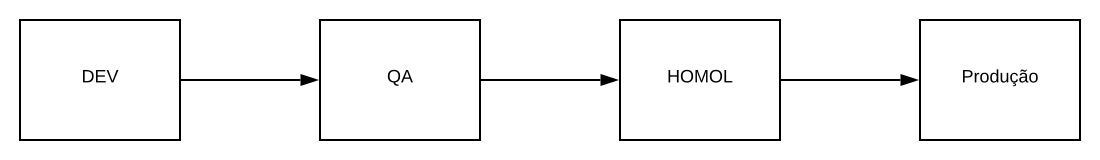
\includegraphics[width=15cm]{enviromentStream.jpeg}
        \caption{Fluxo de ambientes}
        \label{Imagem:1}
      \end{figure}

    \section{Automatizando testes de qualidade}
      Para otimizar a execução dos testes, e facilitar o trbalho dos testadores,
      podemos automatizar os testes que realizamos no sistema, para que sempre que
      uma funcionalidade nova, uma melhoria, uma alteração ou uma correção for
      implementada podemos realizar novamente todos os testes no sistema
      automaticamente. Desta forma, não consumimos tanto tempo dos testadores e
      garantimos que o tudo no nosso sistema continua funcionando da forma que
      esperamos. A fase de automação dos testes, é importante ser realizada assim
      que o requisito for homologado, com a homologação, estamos mais certos que o
      requisito está aderente com o negócio e por causa da etapa de testes, temos
      todos os princípais cenários que presisam ser garantidos, desta forma podemos
      montar testes automatizados para após homologado, qualquer alteração que seja
      realizada nos ambientes de \textbf{QA} e adiante, inicie os testes e garanta
      que os cenários de risco continuem não apresentando problemas para o sistema. \newline
      Os testes devem estar diretamente vinculados com o \textit{deploy} para os
      ambiente, ou seja, é importante que seja um processo do \textit{pipeline},
      onde todo \textit{deploy} realizado, rode novamente todos os testes, em cada
      um dos ambientes, pois desta forma, conseguimos averiguar se alguma alteração
      no sistema impactou em alguma parte que não estavamos prevendo e com essa
      descobertra, conseguimos uma visão mais detalhada do quanto o nosso sistema
      está estruturado, auxiliando nas decisões de arquitetura.

  \chapter{Como adquirir escalabilidade?}
    Conforme o nosso sistema vai aumentando, mais usuários vão utilizando ele,
    mais funcnionalidade ele possui, e mais poder computacional ele necessita.
    Garantir que um sistema se mantenha no ar é uma tarefa complicada, embora
    estejamos desenvolvendo o sistema da melhor forma possível, realizando testes
    na maioria dos cenários e evoluindo a arquitetura para se adequar a atual
    realidade do sistema, não conseguimos prever tudo, e muitas vezes, quando
    mais precisamos que ele funcione, ele apresenta algum problema. Muitas vezes
    podemos subestimar alguma situação ou superestimar outra situação, e se não
    estivermos preparados para os imprevistos, a qualidade de nosso produto pode
    cair e a confiança dos nossos usuários diminuir. \newline
    Vamos imaginar, que a empresa que utilizamos como exemplo anteriormente,
    conseguiu criar um computador base, que atendende muitas necessidades do seus
    clietes, devido a isso, o número de pedidos aumentou, e a empresa teve que
    contratar mais vendedores, mais colaboradores da área técnica e a equipe de
    \textit{marketing} está com várias idéias para novos produtos. O sistema
    nessa situação vai estar constantemente executando vendas, assim como vários
    projetos serão criados, e várias notificações deverão ser disparadas. Certo
    dia, a utilização no sistema foi tão intensa, que o sistema não enviou mais
    notificações durante dois minutos, estes dois minutos foi o suficiente para
    que a área técnica não analisasse três projetos, estes projetos que a equipe
    de \textit{marketing} tinha uma grande expectativa, o tempo passou foi gerado
    o conflito entre as duas áreas, e foi identificado este erro no sistema,
    agora o momento para a produção dos produtos base se perdeu, este conflito
    abalou as duas áreas e a confiança com o sistema pelos usuários diminuiu.

    \section{Descobrindo os limites do sistema}
      Para nos prepararmos para as situações inesperadas, precisamos descobrir os
      limites do nosso sistema, precisamos tentar fazer o sistema falhar em um
      ambiente controlado, antes que ele falhe em produção, quando os nossos usuários
      estiverem utilizando. Entender que nosso sistema tem limites e que ele está
      sucetível a erros é o primeiro passo para descobrirmos como podemos encontrar
      estes erros, devemos utilizar os riscos que mapeamos, e simular diversas vezes
      estes cenários, o que levantamos em nossos requisitos não-funcionais, devem
      ser levado ao extremo, então caso levantamos que um determinado requisito
      deve ter um tempo de resposta de no máximo dois segundos, devemos foçar o
      processamento do nosso sistema para que o tempo de resposta supere dois segundos
      e neste cenário, rodar novamente todos os testes novamente, desta forma nós
      conseguimos ver se o fato do requisito não ser atendido tem algum impacto nos
      critérios que levantamos. Uma vez conseguido simular este cenário, podemos
      mapear os limites do sistema, como nos esforçamos para forçar o sistema a
      funcinoar no seu limite, agora podemos documentar qual é o seu limite e
      analisar se devemos aumentar este limite ou se aceitamos o risco que ele
      representa. \newline
      Definir limites para o sistema é definir novamente os riscos que pretendemos
      aceitar, quando estávamos especificando as nossas funcnionalidades, os riscos
      que mapeamos era com a pespectiva de negócio, nosso objetivo era garantir que
      o que iria ser desenvolvido, gerasse valor e não teria impactos negativos para
      os usuários, agora devemos utilizr estes riscos, em conjunto com os nossos
      requisitos, para mapearmos os limites do sistema. Estamos utilizando o negócio
      para aprender até onde o sistema deve aguentar, e por outro lado, estamos
      utilizando o sistema para aprender o que o negócio precisa e quais riscos
      podemos enfrentar. \newline
      Quando mapeamos os limites do sistema, é importante separarmos os limites por
      funcinalidae e não buscar valores absolutos, mas sim valores estatísticos.
      Por mais testes que realizamos e por mais cenários que simulamos, não podemos
      garantir que em um situação extrema, o sistema vai se comportar sempre da
      mesma forma. Como estamos buscando o extremo, e esperando que o que desenvelvemos
      pare de funcinoar, por mais que tenhamos uma idéia de qual parte do sistema
      vai falhar, não é garantido que as nossas expectativas sempre se cumpram,
      realizando o mesmo teste mais de uma vez, podemos ter diversos retornos
      diferentes. Por este motivo, é interessante, com base na importância da
      funcionalidade, estipular uma quantidade de testes para cada situação extrema,
      com base nos retornos gerados, podemos documentar o que aconteceu e qual foi
      a frequência deste ocorrido, pois caso algum dia venha a ocorrer em produção,
      já temos mapeado os princípais problemas ou uma vez que, produção comece a
      trablhar no limite do sistema, já sabemos o que é mais provável de ocorrer.
      Para armazenarmos os testes que ocorreram, é importante colcoar anotar a
      funcionalidade que testamos, o cenário que estava o sistema e quais foram
      resultados com as porcentagens. Na tabelas nove e dez, exemplificamos está análise
      utilizando a funcnionalidade exemplo de "Cadasto de produtos". \newline

      \begin{table}[h!]
        \centering
        \begin{tabular}{|c|p{10cm}|}
          \hline
          \textbf{Funcionalidade} &
          Cadasto de produtos \\ \hline
          \textbf{Cenário} &
          O processamento do servidor utilizado para a funcnionalidade se encontra
          com 95\% de uso. \\ \hline
          \textbf{Resultado} &
          Em 89\% do cadastro novos projetos, a notificação demorou aproximadamente
          três segundos para aparecer. \\ \hline
          \textbf{Resultado} &
          Em 96\% do cadastro dos novos projetos, levou um aproximadamente dois
          segundos para realizar a criação do projeto. \\ \hline
        \end{tabular}
        \caption{Exemplo de análise de limite de sistema - limite de processamento}
        \label{Tabela:9}
      \end{table}

      \begin{table}[h!]
        \centering
        \begin{tabular}{|c|p{10cm}|}
          \hline
          \textbf{Funcionalidade} &
          Cadasto de produtos \\ \hline
          \textbf{Cenário} &
          Realizado 500 criações de novos projetos ao mesmo tempo. \\ \hline
          \textbf{Resultado} &
          Em 98\% dos cadastros a concexão com o banco de dados foi perdida ao tentar
          inserir os produtos. \\ \hline
        \end{tabular}
        \caption{Exemplo de análise de limite de sistema - limite de requisições}
        \label{Tabela:10}
      \end{table}

      As análises devem ser feitas em um ambiente que seja uma cópia perfeita de
      produção, sempre que algo for entregue em produção, deve ser automaticamente
      replicado para este ambiente, vamos chamá-lo de \textbf{CHAOSPROD} (produção
      caótica). \newline
      Estas análises são prevendo cenários adversos, imaginando situações inesperadas,
      por este motivo, é interessante realizar estas análises sempre após que um
      requisito for entregue em produção, desta forma, conseguimos maior produtividade
      na entrega dos requisitos em desenvolvimento, e uma vez que ele tenha sido
      homologado, e temos o retorno de como os usuários estão utilizando o sistema,
      conseguimos realizar as análises nos baseando não somente no que mapeamos como
      risco, mas também com base em como o usuário está utilizando o sistema e no
      \textit{feedback} que estamos tendo com eles, seja esse \textit{feedback} dito
      diretamente pelo usuário ou através de alguma análise realizada em produção.

      \begin{figure}[!h]
        \centering
        \includegraphics[width=15cm]{enviromentStream_CHAOSPROD.jpeg}
        \caption{Fluxo de ambientes com CHAOSPROD}
        \label{Imagem:2}
      \end{figure}

    \section{Desenvolvendo estratégias de escalabilidade}
      Uma vez identificado os nossos limites, devemos criar estratégias para lidar
      com elas, ser aumentar o poder de processamento dos nossos servidores,
      migrar a nosso aplicação para um banco de dados mais robusto, melhorar o
      desenempendo da funcnionalidade desenvolvida através do código, existem
      várias ações que podemos tomar, para podermos enfrentarmos os riscos que
      mapeamos. \newline
      Para cada cenário que mapearmos precisamos criar um plano, para caso esta
      situação venha a ocorrer. Este plano, deve estar atrelado diretamente a
      importância da funcionalidade e os impactos que sua execução irá gerar,
      devemos considerar os gastos financeiros, o tempo que o plano vai demorar
      para ser executado, os times que irão atuar nele, as áres de negócio que vão
      ser impactadas, como devemos avisar os usuários, entre outras ações. Com a
      realização deste plano, nos preparamos para o imprevisto, caso algum dos
      cenários que mapeamos aconteça, já vamos estar preparado, embora não sabemos
      exatamente o que vai acontecer, temos a probabilidade de cada situação. Podemos
      tambem nos antecipar a esse limite, caso a funcnionalidade seja muito importante
      para o negócio, e identificamos que o limite identificado pode ser atingido,
      podemos trabalhar para aumentá-lo, como sabemos aonde precisamos melhorar,
      basta realizar uma exploração mais aprofundada da melhor forma que podemos
      aumentar este limite. Outro ponto de destaque, é que conseguimos adaptar o
      nosso sistema conforme as necessidades de negócio, caso um determinada
      funcnionalidade necessite de mais processamento, podemos alocar mais servidores
      para esta funcnionalidade, caso um não tenhamos os servidores disponíveis,
      podemos aumentar nosos servidores de forma horizontal, caso não haja verba
      disponível, para aumentar a quantidade de servidores, podemos desativar uma
      funcnionalidade menos importante para realocar os recursos para a funcionalidade
      de maior importância, desta forma, assim que este periodo de maior necessidade
      passar, reativamos a funcnionalidade antiga. \newline
      Para cada caso devemos estruturar uma estratégia e devemos utilizar de métricas
      no ambiente de produção para supervisionar a saúde do ambiente e anteciparmos
      algum tipo de erro. Devemos monitorar o armazenamento já utilizado pelo nosso
      sistema, para caso ele esteja no fim, podemos aumentar o nível de armazenamento
      ou excluir registros antigos, devemos monitorar os nossos servidores, para
      caso algum deles estejam começando a apresentar defeito, ou algum conjunto
      de servidores estejam sendo mais utilizados que outros, assim podemos realocar
      as nossas funcnionalidades em servidores diferentes e aprendemos qual parte
      do sistema utiliza maior quantidade de recursos dos nossos servidores. Podemos
      utilizar diversas acompanhamentos e implementar diversas métricas em nosso
      produto, mas é importante sempre lembrar, que devemos gerar as nossas métricas
      e basear os nossos acompanhamentos com base em como o sistema está sendo
      utilizado, ou seja, é através das necessidades do negócio, que aprendemos
      aonde devemos olhar. Na tabela dez, específicamos como estruturar uma
      estratégia.\newline

      \begin{table}[h!]
        \centering
        \begin{tabular}{|c|p{10cm}|}
          \hline
          \textbf{Funcionalidades} &
          Nome das funcnionalidades que foram impactadas \\ \hline
          \textbf{Cenário} &
          Descrição do cenário em que ocorreu os erros. \\ \hline
          \textbf{Stakeholders} &
          Quais são as áreas de negócio que serão impactadas no cenário descrito. \\ \hline
          \textbf{Times} &
          Quais são os time realcionados para a execução deste plano. \\ \hline
          \textbf{Plano} &
          O que deverá ser feito caso produção se encontre neste cenário. \\ \hline
          \textbf{Tempo de Execução} &
          Tempo para a execução do plano. \\ \hline
        \end{tabular}
        \caption{Especificação para estruturação de estratégias}
        \label{Tabela:11}
      \end{table}

      Com o ambiente de \textbf{CHAOSPROD}, conseguimos descobrir os limites do
      sistema, com o ambiente de produção, conseguimos descobrir como o sistema é
      utilizado, é através dos usuários, e da persepção de valor gerado para eles
      e para o negócio que devemos basear as nossas prioridades e ajustar a
      importância das nossas funcionalidades. Com está visão podemos tomar a decisão
      aonde precisamos testar mais, e também onde precisamos de maior supervisão,
      embora estamos constantemente procurando por erros, não estamos livres de
      falhas, erros em produção vão acontecer. É nestas horas que as ferramentas
      que implementamos para supervisionar o sistema tem sua maior utilidade, é
      através delas que vamos descobrir o que aconteceu e uma vez descoberto, vamos
      utilizar este ocorrido como aprendizado, alem de resolver o problema, vamos
      identificar o porquê ele aconteceu, se realmente resolvemos o problema ou
      mitigamos, se ele pode acontecer e como podemos nos preparar para ele. Este
      erro pode se tornar mais um teste automatizado para ser realizado durante os
      desenvolvimentos ou pode se tornar mais uma análise a ser feita em
      \textbf{CHASOPROD}. De toda forma, ele se tornou um aprendizado para o produto
      e agora faz parte de um cenário que estamos prevendo, pode ser que ele
      aconteça novamente mas desta vez estaremos preparados.

  \chapter{Como manter o seu produto?}
    Para assegurar que o produto continue disponível, gerando valor, confiável
    para o usuário e que ele continue evoluindo junto com o negócio, nós
    precisamos enxergar a saúde do produto. Enxergar a saúde do produto não quer
    dizer apenas analisar questões do sistema como, desempenho, \textit{bugs},
    quantidade de armazenamento e entre outros. Nós precisamos vizualisar como o
    sistema está impactando o negócio, qual o valor que ele está produzindo e
    qual a persepção do usuário durante a sua utilização, precisamos além de
    captar se o sistema ainda está funcionando, de um ponto de vista operacional,
    temos que verificar se ele ainda está funcnionando para o negócio, temos que
    garantir todo dia que ele seja um facilitador para os usuários e não um
    problema e principalmente, precisamos sempre verificar se o sistema está indo
    de encontro com os objetivos do negócio. \newline
    Para conseguirmos estes ensumos, precisamos primeiramente garantir a confiança
    do usuário, eles precisam estar seguros nas ações que eles vão realizar no
    sistema e caso uma melhoria mude a forma que eles realizam as suas atividades,
    é importante informar os usuários o motivo desta alteração e apresentar o
    objetivo da empresa com a mudança do processo. Um usuário informado com
    confiança que o sistema funciona e atende as necessidades dele, se torna
    um colaborador do sistema, é através do \textit{feedback} dele que conseguimos
    mapear as melhorias que devemos realizar e como realizar as comunicações de
    novas implementações. Com base no como o usuário está utilizando o sistema
    é que conseguimos melhorar os nossos testes automatizados e garantir cada vez
    mais qualidade para o nosso produto, o negócio está sempre em constante
    mudança, então precisamos sempre adaptar as nossas funcionalidades para essas
    mudanças. Através dessas mudanças, novos requisitos vão surgindo, novos
    limites serão encontrados e novos riscos irão surgir, com isso mais escolhas
    e mais testes serão necessários para garantir que o sistema continue
    disponível e aderente ao negócio.

    \section{Ouvindo os usuários}
      Há diversas ações que podemos realizar para conseguirmos captar as percepções
      do usuário. A primeira delas é perguntar diretamente para eles, utilizar o
      a opinião de cada usuário para tentar identificar um censo comum, buscando
      entender se o produto está aderente ao negócio, melhorias que devem ser
      implementadas e novas funcnionalidades que devem ser desenvolvidas, todos
      lembrando de classificar a importância de cada nova funcnionalidade ou de
      cada novo requisito. Nestas perguntas é essencial que seja identificado tambem
      questões de usabilidade do que já foi desenvolvido, identificar se as
      operações que eles realizam estão com um bom tempo de resposta, se o
      \textit{layout} não está confuso, se a forma que eles estão interagindo com
      as funcnionalidades faz sentido para eles, se houve algum \textit{bug} ou
      situação que alguma operação não funcionou como o esperado. Através destas
      perspectivas é que conseguimos garantir que os usuários estão satisfeitos
      ao utilizar o sistema. \newline
      Outra ação que devemos realizar para verificar a interação do usuário com o
      sistema é criar métricas no sistema que informe como ele está sendo utilizado.
      Podemos medir o tempo que um usuário leva para realizar uma operação, para
      verificar se determinada operação está com um bom desempenho, quantidade de
      cliques em tela, para verificar se o usuário precisa realizar muitas atividades
      para concluir o seu objetivo, campos em um formulário, para identificar se
      todas as informações ainda fazem sentido o usuário preencher, assim podemos
      ou automatizar o preenchimento de alguns campos ou até mesmo remover eles.
      Para cada funcnionalidade devemos elaborar quais métricas produzir para
      conseguir supervisionar a interação do usuário com o sistema e identificar
      um \textit{bug} durante a utilização do usuário antes mesmo que ele reporte
      o problema para o suporte. Outra análise que podemos fazer com esses dados é
      a de verificar se determinada funcionalidade está apresentando sinais de
      defeito, podemos avriguar por exemplo, que determinada funcnionalidade nos
      ultimos três dias, está apresentando maior lentidão em sua execução. Com
      essa informação podemos investigar se esta lentidão está ocorrendo por causa
      de alguma implementação recente, se um servidor está apresentando defeito,
      se os usuários estão realizando mais requisições para está funcionalidade,
      se a distribuição de processamento nos servidores está aderente a utilização
      dos usuários para cada funcionalidade, entre outras análises. Podemos ver que
      somente este dado, nos abriu diversos pontos de análise, que combinando com
      outras métricas, podemos encontrar a origem do problema, antes mesmo que o
      usuário perceba. Conseguimos assegurar que o sistema se mantenha disponível
      e conseguimos manter a confiança do usuário no produto.

    \section{Aprendendo com os erros}
      Com o frequentemente acompanhamento das funcnionalidades, vamos conseguir
      diversos erros cometidos no produto, um \textit{layout} confuso, algum
      \textit{bug} devido a alguma implementação, um requisito levantado de
      forma errada, gerando uma funcnionalidade funcionando de forma errada, um
      limite que foi alcançado, um risco que não deveriamos ter aceito, pode
      acontecer diversos erros, mesmo com nosso monitoramento contínuo, e o nosso
      desenvolvimento centrado no negócio. O fato de estarmos monitoramendo o nosso
      produto e de desenvolvermos as funcnionalidades centrado no negócio, é o que
      vai nos fazer perceber os nossos erros mais rápido, e também vai nos auxiliar
      a encontrar a solução de forma mais rápida. Uma equipe que entende o negócio,
      sabe os requisitos de cada funcionalidade, sabe os riscos que aceitamos,
      conhece os limites do sistema e consegue monitorar a saúde do produto, tem
      completa capácidade de resolver os problemas e aprender com eles. \newline
      Quando nos deparamos com algum problema em produção, devemos analisar ele
      imediatamene, envolvendo todas as pessoas da equipe que tem realação com o
      acontecido, seja porque trabalhou na funcnionalidade ou as métricas apontram
      que é necessário a participação de um equipe especifica, como por exemplo a
      equipe de infraestrutura, é necessário juntar todos os envolvidos para que
      possamos realizar a análise de forma conjunta e identificar a tratativa de
      uma forma ágil. No momento da análise, é importante lembrar que não há
      culpados, devemos focar na solução do problema, depois de solucionado, é
      importante documentar o ocorrido com a solução que foi realizada e a origem
      do problema. Quando aprendemos com os nossos erros e não repreendemos o
      time por um erro cometido, conseguimos garantir que qualquer problema que
      ocorra, os membros do nosso time não vão sentir medo de reportar e todos vão
      trabalhar em conjunto para resolver o ocorrido. Após resolvido o problemo,
      devemos mapear o que podemos desenvolver para supervisionar o sistema com o
      objetivo de identificar sinais que o erro vai voltar a ocorrer e que caso
      ele ocorra novamente, facilite a nossa análise para a sua resolução. \newline

      \begin{table}[h!]
        \centering
        \begin{tabular}{|c|p{10cm}|}
          \hline
          \textbf{Funcionalidades} &
          Nome das funcnionalidades que foram impactadas. \\ \hline
          \textbf{Cenário} &
          Descrição do cenário em que ocorreu os erros. \\ \hline
          \textbf{Stakeholders} &
          Quais são as áreas de negócio que foram impactadas no cenário descrito. \\ \hline
          \textbf{Problema} &
          Descrição do problema que ocorreu. \\ \hline
          \textbf{Origem do Problema} &
          O que foi que causou o problema descrito. \\ \hline
          \textbf{Equipes Envovidas} &
          Quais equipes foram envolvidas para a resolução. \\ \hline
          \textbf{Solução} &
          O que foi realizado para resolver o problema. \\ \hline
          \textbf{Novos Desenvolvimentos} &
          O que deve ser desenvolvido para monitorar o cenário descrito com o
          objetivo de nos alertar ou facilitar a análise caso o erro volte a
          acontecer. \\ \hline
        \end{tabular}
        \caption{Especificação para documentação de resolução de problemas}
        \label{Tabela:12}
      \end{table}

      Vale lembrar que um erro, não é somente um mau funcionamento de alguma
      funcionalidade, mas sim qualquer impacto negativo para o negócio. Uma
      funcionalidade que não esteja aderente com as necessidades do usuário, deve
      ser tratada conforme descrevemos anteriormente, todos os envolvidos devem
      se reunir e discutir o que deve ser feito para atender as necessidades do
      usuário. Muitas vezes neste caso, os requisitos irão sofrer alterações e o
      teremos que refazer alguma determinada parte de uma funcionalidade, esta
      alteração deverá gerar novos testes automatizados e a arquitetura construída
      terá que se adaptar a estas mudanças, podendo ter que mudar um componente
      inteiro para garantir a aderência ao negócio.

    \section{Testes automatizados como ferramenta de aprendizado}
      Conforme vamos realizando mudanças no produto, seja proveniente de algum erro,
      por mudanças no negócio ou na implementação de alguma melhoria, devemos produzir
      novos testes automatizados para garantir que os novos requisitos dessas mudanças
      estejam sendo testados e garantidos. \newline
      Alem de garantir a qualidade de nossos, os testes eles tem a funlção de servir
      como base de conhecimento, é a partir deles que podemos analisar todos os
      processos que desenvolvemos para o negócio e explicar o funcionamento das
      funcnionalidades. Nos testes automatizados temos sempre como o usuário vai
      interagir com o sistema, onde verificamos se todos os tipos requisitos estão
      sendo garantidos, funcionais, não-funcionais e inversos, conseguimos demonstar
      tudo o que foi feito para garantir a qualidade das funcnionalidades assim
      como o seu funcionamento. Desta forma, conseguimos utilizar os testes automatizados,
      como apresentção do produto como todo, seja para um novo membro da equipe ou
      para um novo usuário, podemos demonstrar o funcionamento de uma nova funcnionalidade,
      para os usuários envolvidos, podemos explicar como funciona um determinado
      processo da empresa. Conseguimos através destes testes, uma grande fonte de
      conhecimento onde com a utilização de um versionador de código, conseguimos
      apresentar as mudanças que foram realizadas na utilização das funcionalidades.
      Através dos testes, conseguimos já prever se uma determinada implantação pode
      gerar algum erro para os usuários, como podemos observar todo um processo sendo
      realizado, conseguimos já na etapa de desenvolvimento averiguar se a solução
      está aderente as necessidades do negócio, verificando se esta nova implementação
      não dificultou o processo que os usuários já estão realizando ou se gerou algum
      impacto em outra parte do sistema, que pode ser visto como um erro para o
      usuário. Conseguimos validar nos testes automatizados, se as mudanças realizadas
      estão seguindo as mudanças que o negócio está sofrendo, como o time tem um
      grande entendimento do negócio e está realizando seus desenvolvimentos com
      foco nos objetivos do negócio, podemos verificar o fluxo que será executado
      pelos usuários nos testes automatizados e validar se as mudanças que ocorreram
      no negócio foram refletidas corretamente para o sistema. \newline
      Devemos ficar atentos as mudanças no negócio, um requisito pode mudar conforme
      o tempo for passando, e nestes casos, ele pode conflitar com o \textit{core}
      do que desenvolvemos, quando isto ocorrer, devemos análisar se realmente faz
      sentido realizar está alteração no sistema ou se devemos começar a construção
      de um novo produto pois, dependendo da mudança, podemos ter que alterar muito
      a forma que o produto funciona, assim gerando muitos riscos na implementação
      dessa nova mudança, os requisitos que mapeamos até então e os testes que
      geramos não estão mais aderentes ao que o negócio está se tornando e muitas
      vezes adaptar o sistema por completo é mais trabalhoso do que desenvolver um
      novo, desta forma conseguimos já na concepção do novo produto, atender os
      novos requisitos e desenvolver funcnionalidades mais aderentes com o caminho
      que negócio está trilhando. Para identificar se a algum ocorrido se trata de
      um erro ou de uma mudança, devemos análisar quanto tempo implementamos os
      requisitos que estão mudando, uma mudança em uma implementação recente, pode
      siginificar um erro ao levantarmos os requisitos, devemos analisar a situação
      em que a sociedade se encontra, pois pode ocorre que algum fator externo, como
      uma nova lei, redefinição de processo, fusão ou aquisição de alguma empresa,
      possa ocasionar em uma mudança, onde nesses casos os requirementos mudaram
      de repente.

  \chapter{Resultados da proposta}
     Ao desenvolver um produto, muitas vezes focamos apenas em requisitos
    funcionais, nos concentramos em entregar o máximo número de funcionalidades
    para os usuários e esquecemos dos requisitos não-funcionais. Conforme apresentado
    no trabalho Quality Attributes and Service-Oriented Architectures
    \cite{O'BrienQualityAttributes2005}, os requisitos não-funcionais estão diretamente
    ligados com a qualidade de nosso \textit{software}, questões como performance,
    usabilidade, segurança e enre outros, são requisitos que garantem que o nosso
    produto funciona e que as nossas funcionalidades desenvolvidas, estão aderentes
    com o negócio. \newline
    Um produto de qualidade deve estar sempre aderente ao negócio, os usuários devem
    conseguir utilizar o sistema e sentir que as necessidades deles estão sendo
    atendidas, eles devem sentir segurança a utilizar o sistema e as funcionalidades
    devem ter um tempo de resposta razoável, para que eles se sintam a vontade ao
    realizar as suas atividades e para que a experiência do usuário não se torne
    frustante. É importante sabermos que não vamos conseguir atender todos os
    requisitos e que teremos que enfrentar riscos no nosso produto, e conforme
    apresentado no The Architecture Tradeoff Analysis Method \cite{KazmanTheArchitecture1998}
    com base nos riscos que analisamos, devemos buscar remodelar a arquitetura que
    desenvolvemos para o nosso produto para que o nosso produto continue com a
    mesma qualidade e possamos mitigar, resolver ou conviver com esses riscos.
    A experiência do usuário e o valor que o produto está gerando para o negócio,
    está diretamente atrelado a qualidade que cada funcnionaliade foi desenvolvida
    e quais os riscos que estamos convivendo, é importante sempre revalidar com o
    negócio, se o que está desenvolvido continua aderente, se algum risco que
    estamos convivendo deveria ser mitigado e com essas análises, se devemos
    investir em reformular a arquitetura montada, para se adaptar as novas definições,
    desenvolver uma nova funcionlidade, atender mais alguma necessidade do negócio
    ou se devemos começar a desenvolver um novo produto pois, o negócio está
    sofrendo diversas alterações que estão descaracterizando o produto desenvolvido
    e que o objetivo do sistema que contruímos foi cumprido e agora a empresa possui
    um novo objetivo. \newline
    Quando desenvolvemos nosso produto em conjunto com o negócio, conforme apresentado
    no Domain Driven Design \cite{DomainDrivenDesign} conseguimos criar uma linguagem
    que será utilizada para que as áreas de negócio e o time de desenvolvimento
    consigam se comunicar e que desta forma, o time de desenvolvimento consegue
    captar melhor os requisitos das funcionalidades e os usuários conseguem
    compreender mais fácilmente como o sistema funciona. Além deste entendimento
    entre as duas partes, é mais criar um código mais limpo, pois os padrões e os
    nomes dos objetos e das entidades serão nomeados baseado em um entendimento
    que todos no time adquiriram ao se comunicar com o negócio. Padrões e estilo de
    desenvolvimento bem definidos entre os membros do time de desenvolvimento facilita
    a compreensão e manutenção do código, como apresentado no Clean Code \cite{CleanCode},
    a maior parte de nosso tempo utilizamos lendo o nosso código do que escrevendo
    linhas novas, e se o código estiver representando o negócio, tanto em sua
    funcnionaliade quanto em sua escrita, ele se torna a documentação do projeto,
    demonstrando como cada parte do sistema funciona e quais requisitos ele está
    atendendo. \newline
    Alem de garantir que o nosso sistema está aderente com o negócio, e que seja
    possível adaptar a sua arquitetura conforme as necessidades do negócio precisamos
    garantir que ele continue em funcionamento em todos os tipos de cituações,
    precisamos utilizar de métricas, produzir \textit{logs}, conversar com o usuário,
    precisamos garantir que caso um problema venha a acontecer, consiguimos supervisionar
    a saúde do ambiente e encontrar a raíz do problema de forma rápida, e após a
    sua resolução, aprender com ele e desenvolver novas formas de supervisão, para
    que consigamos verificar se o sistema está apresentando sinais que o erro vai
    voltar a ocorrer. Com o aprendizado que obtivemos com o erro, agora podemos
    elaborar estratégias para nos preparar para futuras situações, seja aumentar
    a quantidade de servidores durante um determinado período, seja particionar
    mais o processamento de alguma funcionalidade do sistema ou seja até mesmo
    desativar por completo uma funcionalidade que não está mais sendo utilizada,
    mas ainda consome recursos computacionais, através do negócio e com as situações
    que enfrentamos dia a dia, podemos traçar estratégias, redefinir a nossa
    arquitetura e adquirir maior consciência sobre o negócio como um todo, pois
    desta forma estamos utilzando o negócio para definir o sistema e o sistema
    para aprender sobre o negócio.
